
\section{Empirical Evaluations}
\label{sec:experiments}

In this section, we review the results demonstrating transfer from language to other modalities, and seek to better understand why this occurs and what enables this transfer.
All model sizes are the base model size (12 layers, 768 hidden dimension), unless stated otherwise.
See Appendix \ref{app:experimental_details} for more details on experiments.

\subsection{Can pretrained language models transfer to different modalities?}
\label{sec:transfer}

We investigate if the self-attention and feedforward layers -- the main body -- of a pretrained transformer can be applied to a classification problem in a different modality without finetuning.
To do this, we apply our base procedure as described above, where the input embedding layer, output readout layer, and layer norm parameters are finetuned.

Our results are shown in Figure \ref{fig:main_result} and also summarized below in Table \ref{table:main_result}.
We compare to state-of-the-art from literature when available (full transformer on ListOps, CIFAR-10 LRA, and Remote Homology; LSTM on Remote Homology).
Note the benchmarks from literature do not include decimal points, so for those numbers we report without a decimal.

We find that across all seven tasks considered, FPT achieves comparable performance to the fully trained transformer benchmarks.
We believe these results support the idea that these models are learning representations and performing computation that is agnostic to the modality.
We also note that both transformer variants significantly outperform LSTMs on some tasks, particularly ListOps and CIFAR-10 LRA, which have long sequence lengths of 512 and 1024, respectively.

On the two bit tasks (Memory and XOR), the models achieve 100\% performance, i.e. they are able to recover the exact algorithm.
Although our tables show results for $n=5$, we actually find FPT can still recover the exact algorithm on sequence lengths greater than $n=256$ (the elementwise XOR of two bitstrings each of length $256$), hinting that FPT has a fairly large working memory.

\begin{table}[h] 
\begin{center}
\begin{tabular}{c|ccccccc}
\toprule
\textbf{Model} & \multicolumn{1}{c}{\bf Bit Memory} & \multicolumn{1}{c}{\bf XOR} & \multicolumn{1}{c}{\bf ListOps} & \multicolumn{1}{c}{\bf MNIST} & \multicolumn{1}{c}{\bf CIFAR-10} & \multicolumn{1}{c}{\bf C10 LRA} & \multicolumn{1}{c}{\bf Homology} \\
\midrule
FPT & 100\% & 100\% & 38.4\% & 98.0\% & 72.1\% & 38.6\% & 12.7\% \\
Full & 100\% & 100\% & 38\% & 99.1\% & 70.3\% & 42\% & 9\% \\
LSTM & 60.9\% & 50.1\% & 17.1\% & 99.5\% & 73.6\% & 11.7\% & 12\% \\
\bottomrule
\end{tabular}
\end{center}
\caption{Test accuracy of FPT vs fully training transformer on downstream task vs fully training LSTM on downstream task (results are transcribed from Figure \ref{fig:main_result}).} \label{table:main_result}
\end{table}

We highlight a few important points for contextualizing these results.
We find that it can be difficult to fully train a 12-layer transformer on some of these (relatively small) datasets, as training can either diverge/overfit or be unstable.
For CIFAR-10, we report the full transformer results for a 3-layer model; for ListOps and CIFAR-10 LRA we report the number given for the 3-layer model from \cite{tay2020lra}; for Remote Homology we report the number for a smaller 12-layer model from \cite{rap2019tape}.
From an engineering perspective, this makes the full transformers harder to tune since we must choose model sizes that are stable and avoid overfitting -- see Section \ref{sec:generalization} for more analysis.
In particular, the numbers from \cite{tay2020lra} are generated from ``extensive sweeps over different hyper-parameters'' and use task-specific hyperparameters, while we do not tune the hyperparameters for FPT (except for remote homology; see Appendix \ref{app:experimental_details}).
In contrast, we find it is easy to improve the performance of FPT by increasing model size (see Section \ref{sec:size}) -- the CIFAR-10 number for FPT here is for the 36-layer large model.

Furthermore, unlike some other works utilizing transformers for vision, we use minimal spatial bias to emphasize the universal sequential aspect of the problem -- for instance, we do not interleave self-attention and convolution layers.
Note that we also do not use 2D positional embeddings (or other domain-specific techniques), hence providing very weak inductive prior to the model.
Our reasoning for these decisions is to evaluate the ability of transformers to work on arbitrary sequential tasks.

\subsection{What is the importance of the pretraining modality?}
\label{sec:pretraining}

We now compare pretraining on language to other pretraining methods for base model sizes:
\begin{itemize}[leftmargin=*]
    \item Random initialization (Random): initialization of the frozen transformer parameters randomly using the default initialization choices for GPT-2, i.e. without pretraining.
    
    \item Bit memory pretraining (Bit): pretraining from scratch on the Bit Memory task and then freezing the parameters before transferring.
    This allows the transformer to gain supervision working with arbitrary bit strings and performing memory/denoising on independent inputs.
    
    \item Image pretraining (ViT): using a pretrained Vision Transformer \citep{dosovitskiy2020vit} pretrained on ImageNet-21k \citep{deng2009imagenet}.
    Note that the architecture is a bit different, notably not using the autoregressive masking of GPT-2, since ViT is only pretrained on classification tasks (for other details, see Appendix \ref{app:details_pretraining}). 
\end{itemize}

These experiments highlight the significance of pretraining -- as opposed to simply the transformer architecture -- and compare language to other methods of supervision.
Our results are shown in Table \ref{table:random}.
Although the random transformers can achieve surprisingly strong accuracies, there is a considerable gap to using natural language pretraining, such as in MNIST, where random transformers achieve similar performance to a linear classifier on top of raw features (92\%).
Thus we believe that while the transformer architecture might be naturally conducive to these evaluations, the attention mechanisms used to transfer may be nontrivial and not fully specified by the architecture.
We also find that, in addition to performance benefits, language pretraining improves convergence compared to the randomly initialized transformer (see Section \ref{sec:compute_efficiency}).

\begin{table}[h] 
\begin{center}
\begin{tabular}{c|ccccccc}
\toprule
\textbf{Model} & \multicolumn{1}{c}{\bf Bit Memory} & \multicolumn{1}{c}{\bf XOR} & \multicolumn{1}{c}{\bf ListOps} & \multicolumn{1}{c}{\bf MNIST} & \multicolumn{1}{c}{\bf C10} & \multicolumn{1}{c}{\bf C10 LRA} & \multicolumn{1}{c}{\bf Homology} \\
\midrule
FPT & 100\% & 100\% & 38.4\% & 98.0\% & 68.2\% & 38.6\% & 12.7\% \\
Random & 75.8\% & 100\% & 34.3\% & 91.7\% & 61.7\% & 36.1\% & 9.3\% \\
Bit & 100\% & 100\% & 35.4\% & 97.8\% & 62.6\% & 36.7\% & 7.8\% \\
ViT & 100\% & 100\% & 37.4\% & 97.8\% & 72.5\% & 43.0\% & 7.5\% \\
\bottomrule
\end{tabular}
\end{center}
\caption{
Test accuracy of language-pretrained (FPT) vs randomly initialized (Random) vs Bit Memory pretraining (Bit) vs pretrained Vision Transformer (ViT) models.
The transformer is frozen.
}\label{table:random}
\end{table}

Pretraining on bit memory improves performance compared to the random models, but still lags behind training on natural language data.
Furthermore, measured by gradient steps, all models converge faster than the randomly initialized transformers (more details in Section \ref{sec:compute_efficiency}), indicating that all modes of pretraining improve upon random initialization even without considering accuracy.

Additionally, while freezing a vision transformer yields better improvements on CIFAR-10, pretraining on images is not uniformly better; e.g., ViT is worse on protein classification.
One hypothesis is that protein sequences are structured like language, in terms of discrete units of information with a ``grammar'', so transfer from language to proteins may be more natural.
\vspace{2em}

\subsection{How important is the transformer architecture compared to LSTM architecture?}
\label{sec:architecture_results}

In Section \ref{sec:pretraining} we found the transformer architecture can already be fairly effective in this regime, even with only random parameters.
In this section, we consider using a random LSTM architecture instead of the transformer, allowing us to consider the raw effect of architecture and ablating pretraining.
Like FPT, we finetune the input, output, and layernorm parameters for the LSTMs.

\begin{table}[h] 
\begin{center}
\begin{tabular}{c|ccccccc}
\toprule
\textbf{Model} & \multicolumn{1}{c}{\bf Bit Memory} & \multicolumn{1}{c}{\bf XOR} & \multicolumn{1}{c}{\bf ListOps} & \multicolumn{1}{c}{\bf MNIST} & \multicolumn{1}{c}{\bf CIFAR-10} & \multicolumn{1}{c}{\bf C10 LRA} & \multicolumn{1}{c}{\bf Homology} \\
\midrule
Trans.   & 75.8\% &  100\% & 34.3\% & 91.7\% & 61.7\% & 36.1\% & 9.3\% \\
LSTM     & 50.9\% & 50.0\% & 16.8\% & 70.9\% & 34.4\% & 10.4\% & 6.6\% \\
LSTM$^*$ & 75.0\% & 50.0\% & 16.7\% & 92.5\% & 43.5\% & 10.6\% & 8.6\% \\
\bottomrule
\end{tabular}
\end{center}
\caption{Test accuracy of randomly initialized transformers vs randomly initialized LSTM models. Note unlike in Figure \ref{fig:main_result}, the LSTM here is frozen. Frozen LSTMs perform very poorly. LSTM$^*$ represents an LSTM with additional architecture improvements to match the transformers (see below).}\label{table:random_architecture}
\end{table}
\vspace{-.5em}

Our results are shown in Table \ref{table:random_architecture}.
``LSTM'' refers to a 3-layer ``standard'' LSTM with a hidden dimension of 768, matching standard implementations of LSTMs, without residual connections or positional embeddings (see discussion below).
This matches the width of the FPT models, but not the depth or total parameter count (note that LSTMs also do not have positional embeddings).
We find that the self-attention architecture already serves as an effective inductive bias for universal computation, improving significantly over the recurrent LSTM model and comprising most of the improvement in test accuracy from random LSTM to FPT.

Here, we compare the 3-layer ``standard'' LSTM to a 12-layer ``standard'' LSTM.
Note that most LSTM implementations, including the one used in Table \ref{table:random_architecture}, do not feature residual connections and positional embeddings.
We include this comparison to represent the traditional method more faithfully, but add these additional architectural components below.
In the same style of FPT and GPT-2, we do not use a bidirectional LSTM.
Under these model choices, we report the performance of a frozen random 3-layer vs 12-layer LSTM in Table \ref{table:lstm_layers}.
Naively, the 12-layer model is much worse than the 3-layer model, hinting that there is some loss of information by repeated LSTM layers.

\begin{table}[h] 
\begin{center}
\begin{tabular}{c|cccc}
\toprule
\textbf{Layers} & \multicolumn{1}{c}{\bf ListOps} & \multicolumn{1}{c}{\bf MNIST} & \multicolumn{1}{c}{\bf CIFAR-10} & \multicolumn{1}{c}{\bf C10 LRA} \\
\midrule
12 & 16.2\% & 11.7\% & 10.8\% & 10.4\% \\
3  & 16.8\% & 70.9\% & 34.4\% & 10.4\% \\
\bottomrule
\end{tabular}
\end{center}
\caption{Test accuracy of randomly initialized ``standard'' LSTMs varying number of layers with a hidden dimension of 768. The simple 12-layer LSTM achieves only near-trivial performance.}\label{table:lstm_layers}
\end{table}
\vspace{-.5em}

We also experiment with ablating other architectural improvements included with the transformer architecture in Table \ref{table:lstm_layers_residual}.
Once residual connections \citep{he2016resnet} are added, the 12-layer LSTM makes up a lot of the performance drops, hinting that residual connections could make up for loss of information from the LSTM layers which otherwise linearly combine the features.
We also add positional embeddings, which finishes bridging the gap between standard LSTM implementations and the transformer.
Even with these additional benefits, the LSTM still performs worse.
Note that the final 12-layer LSTM has about the same number of trainable parameters as the transformer.

\begin{table}[h] 
\begin{center}
\begin{tabular}{c|cccc}
\toprule
\textbf{Model} & \multicolumn{1}{c}{\bf ListOps} & \multicolumn{1}{c}{\bf MNIST} & \multicolumn{1}{c}{\bf CIFAR-10} & \multicolumn{1}{c}{\bf C10 LRA} \\
\midrule
12-Layer LSTM           & 16.2\% & 11.7\% & 10.8\% & 10.4\% \\
+ Residual Connections  & 16.8\% & 70.9\% & 34.4\% & 10.4\% \\
+ Positional Embeddings & 16.7\% & 92.5\% & 43.5\% & 10.6\% \\
\midrule
Random Transformer      & 34.3\% & 91.7\% & 61.7\% & 36.1\% \\
\bottomrule
\end{tabular}
\end{center}
\caption{Test accuracy of 12-layer randomly initialized ``standard'' LSTMs additional architectures modifications to match transformers: residual connections and positional embeddings.
The bottom row, LSTM with residual connections and positional embeddings, is nearly identical to GPT-2.}\label{table:lstm_layers_residual}
\end{table}

\subsection{Does language pretraining improve compute efficiency over random initialization?}
\label{sec:compute_efficiency}

We investigate compute efficiency by considering the number of gradient steps to converge for FPT vs random transformer models, shown in Table \ref{table:convergence}.
We generally find FPT converges faster, which indicates language pretrainining can yield compute benefits for non-language tasks.
While random transformer models achieve decent test accuracies, in particular when compared to random LSTMs, there is still a considerable gap in the compute efficiency compared to using pretraining.
Note that bit memory pretraining introduced in Section \ref{sec:pretraining} generally falls between the two models, and notably is $6 \times$ slower than FPT on Bit XOR, which is significantly better than random.

\begin{table}[h] 
\begin{center}
\begin{tabular}{c|ccccccc}
\toprule
\textbf{Model} & \multicolumn{1}{c}{\bf Memory} & \multicolumn{1}{c}{\bf XOR} & \multicolumn{1}{c}{\bf ListOps} & \multicolumn{1}{c}{\bf MNIST} & \multicolumn{1}{c}{\bf C10} & \multicolumn{1}{c}{\bf C10 LRA} & \multicolumn{1}{c}{\bf Homology} \\
\midrule
FPT & $1 \times 10^4$ & $5 \times 10^2$ & $2 \times 10^3$ & $5 \times 10^3$ & $4 \times 10^5$ & $3 \times 10^5$ & $1 \times 10^5$\\
Random & $4 \times 10^4$ & $2 \times 10^4$ & $6 \times 10^3$ & $2 \times 10^4$ & $4 \times 10^5$ & $6 \times 10^5$ & $1 \times 10^5$ \\
\midrule
\textbf{Speedup} & $4 \times$ & $40\times$ & $3 \times$ & $4 \times$ & $1 \times$ & $2 \times$ & $1 \times$ \\
\bottomrule
\end{tabular}
\end{center}
\caption{Approximate number of gradient steps until convergence for pretrained (FPT) vs randomly initialized (Random) models. Note that we use the same batch size and learning rate for both models.}\label{table:convergence}
\end{table}

\subsection{Do the frozen attention layers attend to modality-specific tokens?}
\label{sec:attention_maps}

We investigate if FPT attends to semantically meaningful patterns in the data.
We plot the attention weights (i.e. the values of the softmax of query-key dot product) from the first layer.
We show the results in Figures \ref{fig:attn_xor_pretrained} and \ref{fig:attn_memory_pretrained} for the bit tasks.
Note GPT-2 is autoregressive, so the upper right corner of the attention mask is zeroed out.
On these tasks, FPT yields an interpretable attention pattern despite not training the self-attention layers themselves.
We did not find easily interpretable patterns on the other tasks.

\begin{figure}[H]
    \centering
    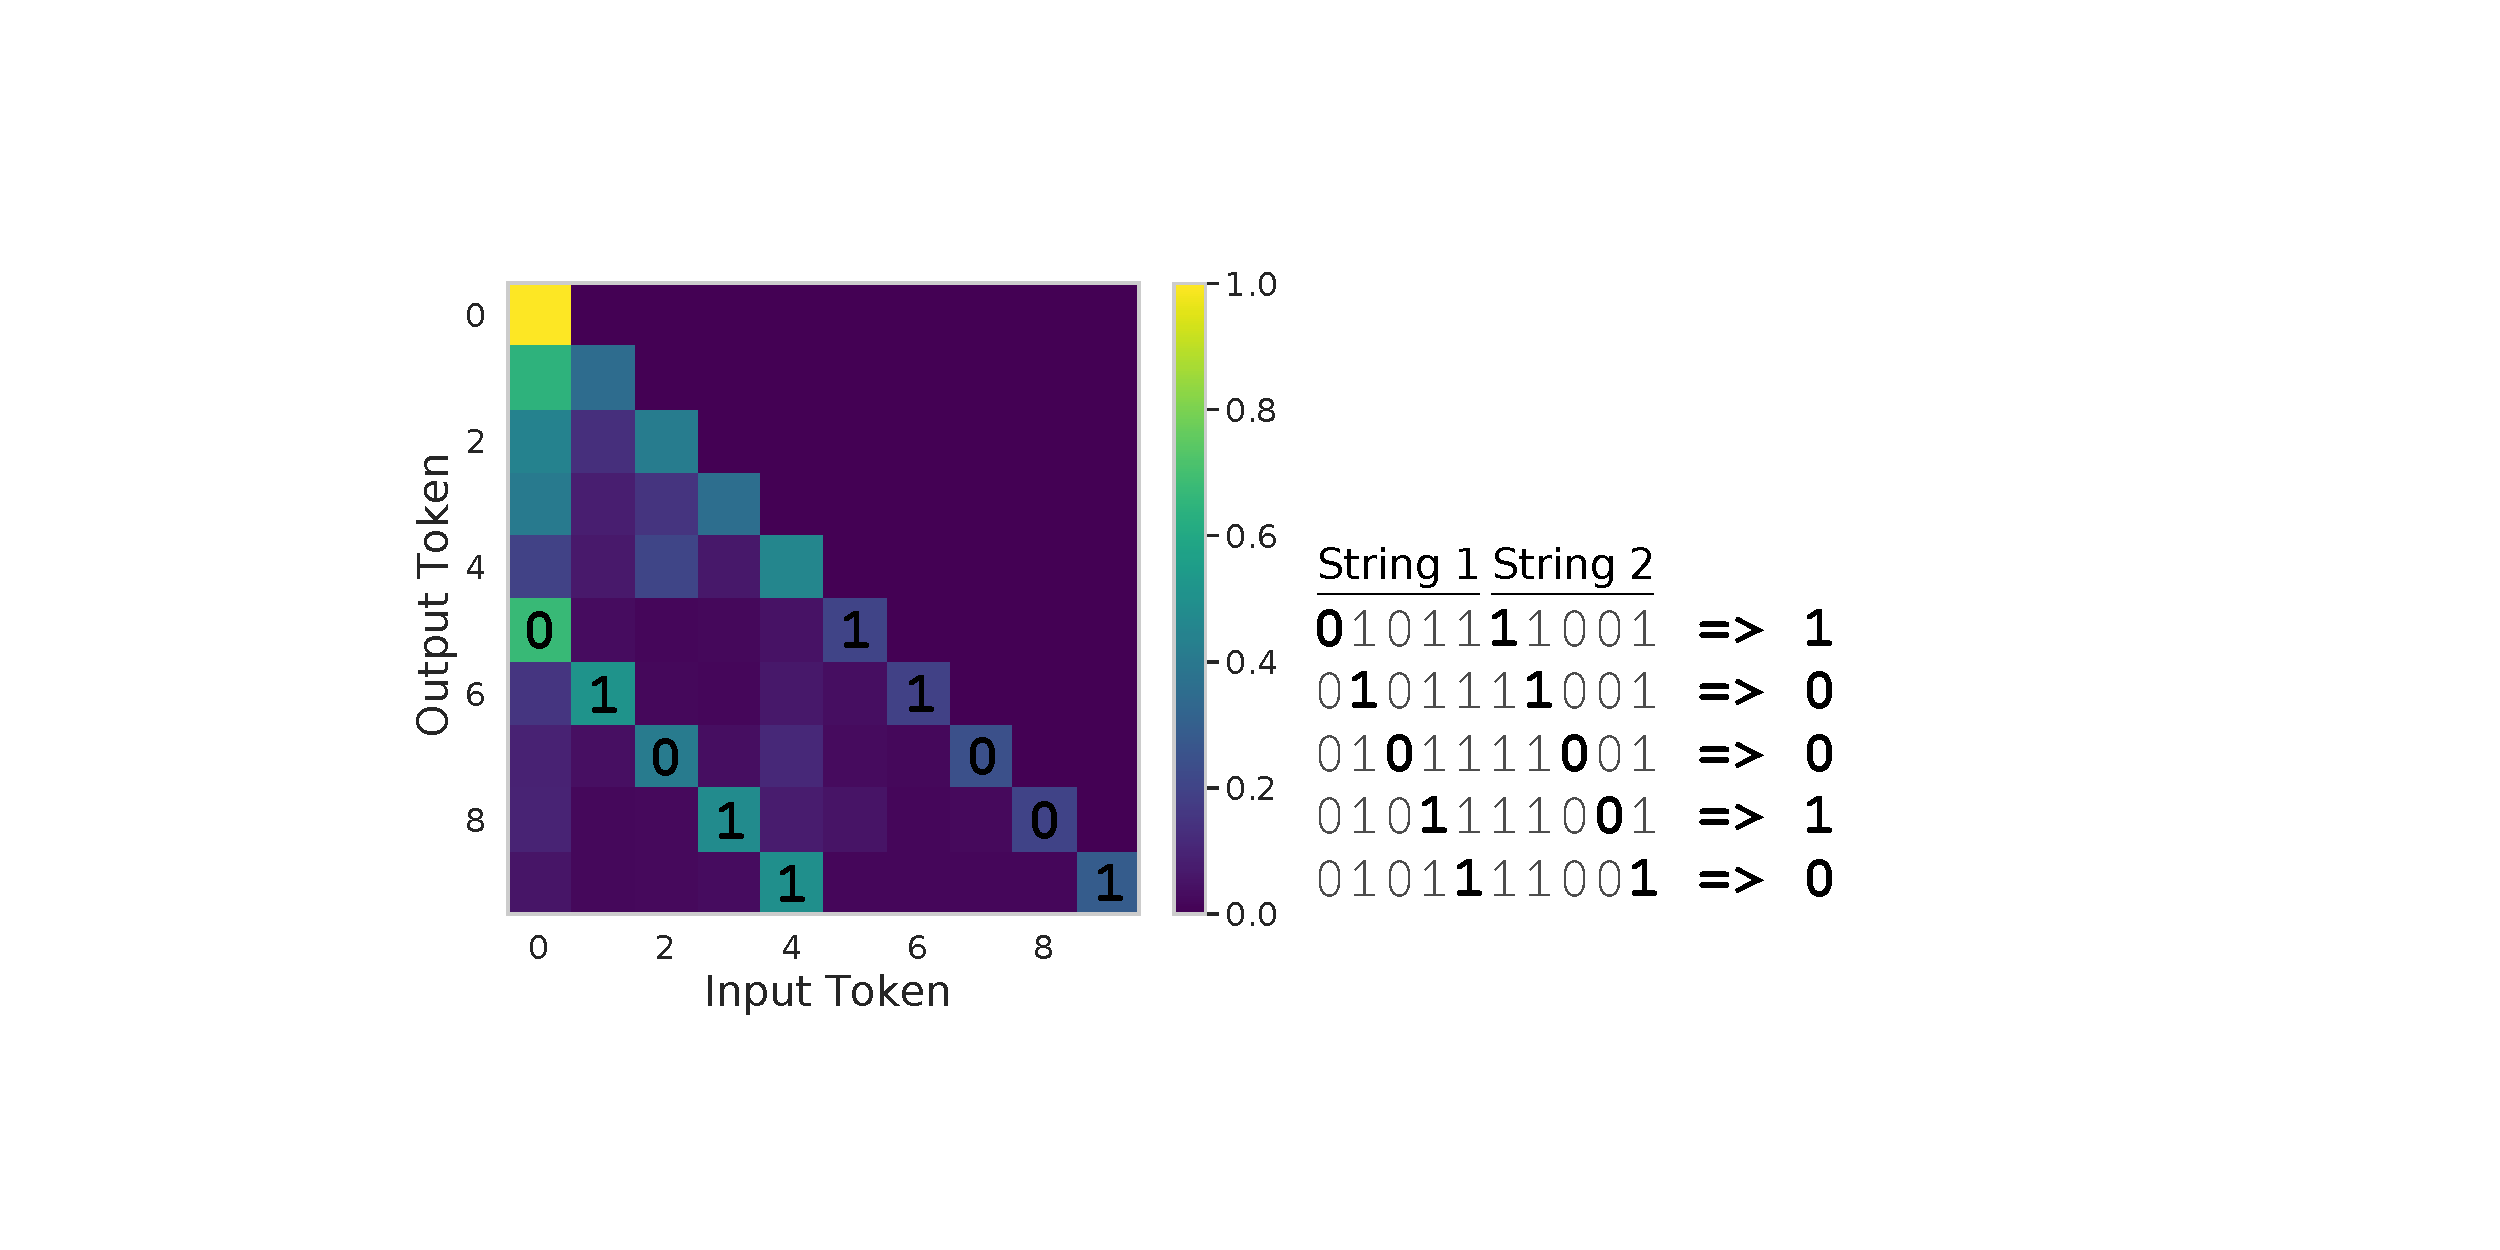
\includegraphics[width=0.55\linewidth]{figures/attention_maps/xor_pretrained}
    \caption{
        On Bit XOR, the model must produce the element-wise XOR of two bitstrings presented sequentially (inputs 0-4 are the first bitstring, inputs 5-9 are the second).
        Each token is one bit.
        FPT learns to attend positionally to the two bits that are XOR'ed by the output token.
    }
    \label{fig:attn_xor_pretrained}
\end{figure}

\begin{figure}[H]
    \centering
    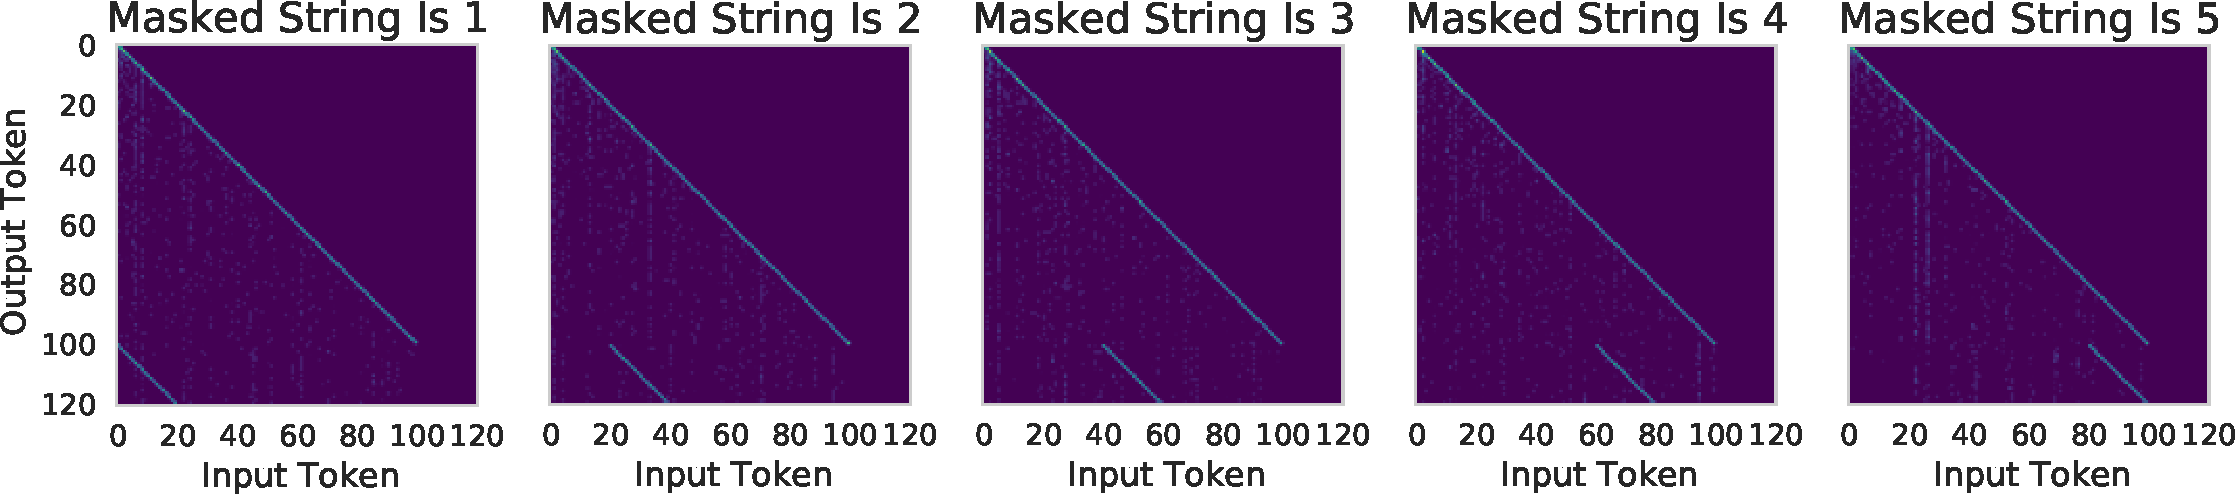
\includegraphics[width=.95\linewidth]{figures/attention_maps/memory_pretrained}
    \caption{
        On Bit Memory, the model must return one of five strings (inputs 0-99) given a masked version of one of the strings (inputs 100-119).
        Each token is 50 bits.
        FPT learns to attend to the correct string based on finding similarity to the inputs, not relying solely on position as in Bit XOR.
    }
    \label{fig:attn_memory_pretrained}
\end{figure}

We also include the attention map for Bit XOR using a randomly initialized transformer (which also solves the task) in Figure \ref{fig:attn_xor_random}.
This model also learns to exploit the diagonal pattern, although the strength is a little weaker.
This indicates that while the random transformer still learns to solve the task, it learns a less semantically interpretable/strong attention pattern.

\begin{figure}[H]
    \centering
    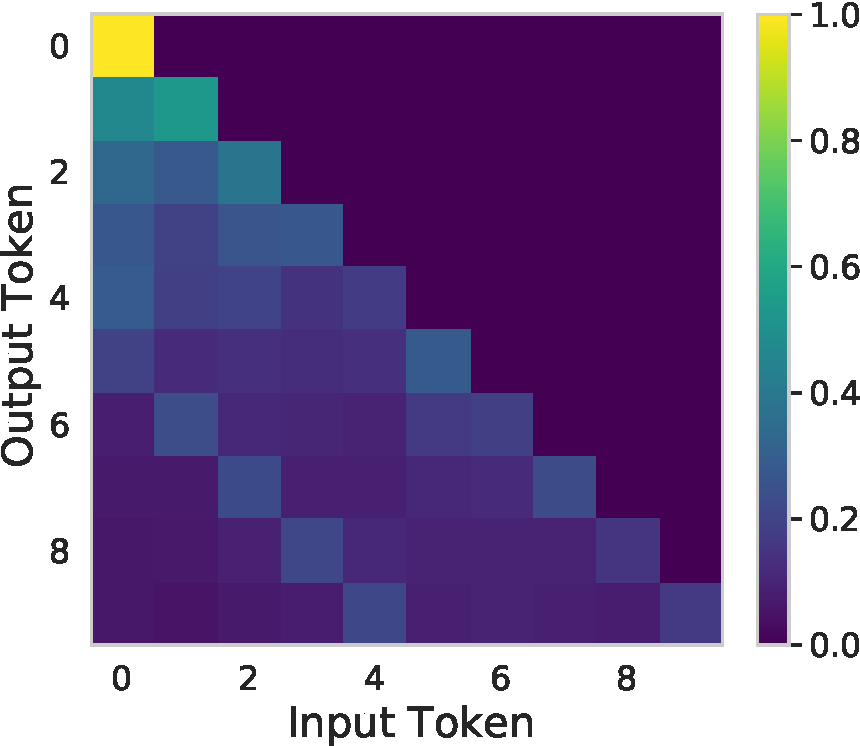
\includegraphics[width=0.3\linewidth]{figures/attention_maps/xor_random}
    \caption{
        A transformer with frozen randomly initialized self-attention layers also learns to correlate the two diagonal elements on Bit XOR, although the magnitude of the diagonals is lower (note the extra attention weights distributed in between the diagonals).
    }
    \label{fig:attn_xor_random}
\end{figure}

\subsection{Does freezing the transformer prevent overfitting or underfitting?}
\label{sec:generalization}

Our general findings are that -- in contrast to their fully trained counterparts -- FPT models underfit the data, which lends them to further improvements by increasing model capacity (see Section \ref{sec:size}).
For example, consider CIFAR-10 LRA, which is maximally difficult due to lack of inductive prior over the sequence (each pixel is fed in as an arbitrary token only ordered by a raster scan) and relatively small dataset (50k images).
In Table \ref{table:generalization}, we show the train/test gap between training FPT vs a 3-layer transformer from \cite{tay2020lra}, which we find to give stronger results than our experiments.
In particular, they are much better than training a 12-layer transformer, which works poorly.
Our results indicate that FPT is generally providing generalizable task representations without causing overfitting, whereas transformers can overfit arbitrarily poorly in low-data regimes (such as for Linformer, which overfit the most out of the architectures tested by \cite{tay2020lra}).
More work can investigate how to increase the model expressiveness, which could yield performance benefits.

\begin{table}[h] 
\begin{center}
\begin{tabular}{c|c|cc}
\toprule
\textbf{Model} & \textbf{\# Layers} & \multicolumn{1}{c}{\bf Test Accuracy} & \multicolumn{1}{c}{\bf Train Accuracy} \\
\midrule
FPT (GPT-2) & 12 & 38.6\% & 38.5\% \\
Vanilla Transformer & 3 & 42\% & 70\% \\
Linformer & 3 & 39\% & 97\% \\
\bottomrule
\end{tabular}
\end{center}
\caption{Train vs test accuracies on CIFAR-10 LRA task.}\label{table:generalization}
\end{table}

% \subsection{How does out-of-modality pretraining compare with in-modality pretraining?}
% \label{sec:in_modality_pretraining}

% We discuss FPT in relation to results from other works evaluating in-modality pretraining for images and protein modeling.

\subsection{Does performance scale with model size?}
\label{sec:size}

We evaluate the efficacy of adding more parameters to these models on CIFAR-10.
Most of the additional parameters are in the transformer layers and are trained during the natural language pretraining phase.
Our results for pretrained and random models are in Table \ref{table:larger_models}.
Unlike fully training a transformer, which exhibits more overfitting and divergence during training with larger models, increasing model size stably increases the capacity of the models.
This result indicates our observations and results are likely to scale as we move towards larger models and higher-data regimes.

\begin{table}[h] 
\begin{center}
\begin{tabular}{c|ccc|cc}
\toprule
\textbf{Model Size} & \multicolumn{1}{c}{\bf \# Layers} & \multicolumn{1}{c}{\bf Total Params} & \textbf{Trained Params} & \multicolumn{1}{c}{\bf FPT} & \multicolumn{1}{c}{\bf Random} \\
\midrule
Small (Base) & 12 & 117M & 106K & 68.2\% & 61.7\% \\
Medium       & 24 & 345M & 190K & 69.8\% & 64.0\% \\
Large        & 36 & 774M & 300K & 72.1\% & 65.7\% \\
\bottomrule
\end{tabular}
\end{center}
\caption{Test accuracy of larger frozen transformer models on CIFAR-10.}\label{table:larger_models}
\end{table}

\subsection{Can performance be attributed simply to better statistics for initialization?}
\label{sec:initialization}

In this section, we ablate taking the layer-wise mean and standard deviation from the pretrained model and using it to initialize a random transformer, in order to ablate if a better initialization scheme via an ``oracle'' standard deviation can recover the performance of FPT.
Note that the GPT-2 initialization scheme initializes parameters as Gaussian; traditionally, the standard deviation is $0.02$ by default.
For clarity, we show the standard deviation by layer for the weights and biases of the attention and feedforward layers in Figure \ref{fig:statistics} for the pretrained models.

\begin{figure}[H]
    \centering
    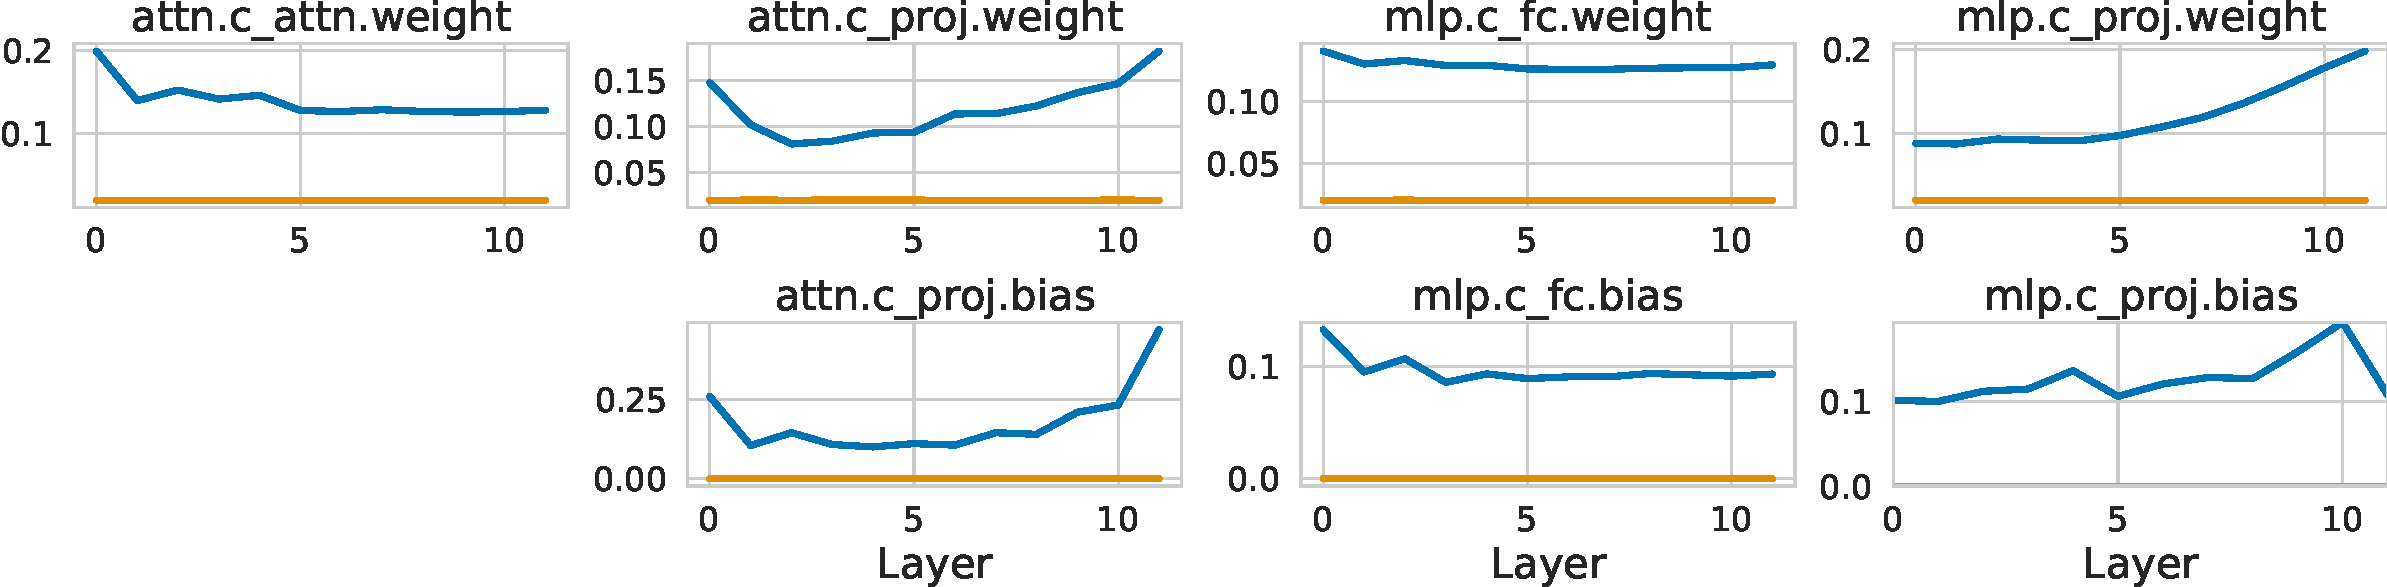
\includegraphics[width=1\linewidth]{figures/statistics/statistics.pdf}
    \vspace{1em}
    
\includegraphics[width=0.6\linewidth]{figures/statistics/stats_legend.pdf}
    \caption{
        Standard deviation of the parameters by layer for the pretrained GPT-2 model versus default initialization hyperparameters ($0.02$ for weights and $0$ for biases).
        % Note that the magnitude of the means tend to be very small ($< 10^{-3}$), so these minimally affect initialization.
    }
    \label{fig:statistics}
\end{figure}

\vspace{-1em}

We show the results using this initialization scheme in Table \ref{table:initialization} (note that all of the weights, biases, layer norm, and positional embeddings are initialized -- both mean and variance -- in this fashion).
This yields better results on most tasks, but does poorly on CIFAR-10.
As a result, we believe the benefits of language pretraining cannot be recovered with a simple better initialization scheme, although we believe future work in transformer initialization could yield different results.

\begin{table}[H] 
\begin{center}
\begin{tabular}{c|ccccccc}
\toprule
\textbf{Initialization} & \multicolumn{1}{c}{\bf Memory} & \multicolumn{1}{c}{\bf XOR} & \multicolumn{1}{c}{\bf ListOps} & \multicolumn{1}{c}{\bf MNIST} & \multicolumn{1}{c}{\bf C10} & \multicolumn{1}{c}{\bf C10 LRA} & \multicolumn{1}{c}{\bf Homology} \\
\midrule
Pretrained & 100\% & 100\% & 38.4\% & 98.0\% & 68.2\% & 38.6\% & 12.7\% \\
Statistics Only & 100\% & 100\% & 37.4\% & 97.2\% & 56.5\% & 33.1\% & 11.0\% \\
Default & 75.8\% & 100\% & 34.3\% & 91.7\% & 61.7\% & 36.1\% & 9.3\% \\
\bottomrule
\end{tabular}
\end{center}
\caption{Test accuracy when initializing parameters with pretrained weights (i.e., FPT) vs randomly initializing parameters according to the mean and variance of the pretrained transformer (Statistics Only) vs random initialization with default parameters (Default).}\label{table:initialization}
\end{table}
\vspace{-1.8em}

\subsection{Can we train a transformer by only finetuning the output layer?}
\label{sec:reservoir}

We consider using FPT solely for naive feature extraction for linear classification, where we fix a randomly initialized input layer and freeze all parts of the model except for the output.
Note that this resembles resevoir computing/echo state networks (see Section \ref{sec:gwt} for discussion).
The model evaluates on every example in the training set once, caches the features, and then we train a linear output layer.
This enables subsequent epochs after the first to run extremely quickly, but does not easily handle dropout/data augmentations, and scales well in terms of number of epochs, but not in dataset size.
Note that this is mathematically equivalent to linear classification.
Our results are shown in Table \ref{table:linear}.
Although we find speedups extremely significant and they obtain nontrivial performance, performance significantly degrades and the models also exhibit overfitting (likely due to lack of regularization; unlike the training of FPT, dropout is not applied).

\begin{table}[H]
\begin{center}
\begin{tabular}{c|c|ccc}
\toprule
\textbf{Task} & \textbf{Speedup} & \multicolumn{1}{c}{\bf Output Only} & \multicolumn{1}{c}{\bf FPT} & \multicolumn{1}{c}{\bf Full Transformer}  \\
\midrule
ListOps      & $500-2000\times$ & 32.8\% & 38.4\% & 38\% \\
CIFAR-10 LRA & $500-2000\times$ & 24.7\% & 38.6\% & 42\% \\
\bottomrule
\end{tabular}
\end{center}
\caption{Training only the output layer as a linear regression problem. Speedup refers to wall clock time per epoch (after the first). Larger models have larger speedups.}\label{table:linear}
\end{table}

\subsection{What is the role of model depth in token mixing?}
\label{sec:model_depth}

One interesting question is the importance of the depth of the transformer for generating representions which ``mix'' tokens: for instance, if there is only one layer and the parameters are random, it is unlikely for the tokens to be mixed well, whereas if there are many layers, there are many chances for the tokens to mix and form interesting representations useful for downstream tasks.
We investigate this on ListOps by considering pretrained vs random models, where we only take the first X layers of the 12-layer pretrained model (i.e. for X=3, we use the first 3 layers of the pretrained GPT-2 model and perform classification from those hidden states).
Additionally, to maximally highlight the importance of the pretrained parameters, we randomly initialize the input layer, and do not train the input or positional parameters.
We first show results are finetuning the output layer and layernorm parameters, and then show only finetuning the output layer.

\textbf{With finetuning layernorm.}
We first investigate this question with finetuning the layernorm parameters (i.e. we finetune only the output layer and the layernorm parameters).
Results are shown in Table \ref{table:depth_ln}.
Both models are unable to do well with only one layer, but the pretrained model performs significantly better than the random model at 2 layers, indicating that while the difference in performance at 12 layers is relatively small, there is a great benefit to using pretrained layers for when considering a small number of layers in that the tokens are ``mixed'' faster.

\begin{table}[h] 
\begin{center}
\begin{tabular}{c|cc}
\toprule
\textbf{Number of Layers} & \multicolumn{1}{c}{\bf Pretrained} & \multicolumn{1}{c}{\bf Random} \\
\midrule
1 & 17\% & 17\% \\
2 & 36\% & 16\% \\
6 & 38\% & 35\% \\
\bottomrule
\end{tabular}
\end{center}
\caption{Test accuracy on Listops while varying model depth and finetuning layernorm parameters. Pretrained layers ``mix'' the tokens faster, performing better at low model depths.}\label{table:depth_ln}
\end{table}

\textbf{Without finetuning layernorm.}
We now investigate this question without finetuning the layernorm parameters, and only finetuning the output parameters, as in the reservoir computing setup in Section \ref{sec:reservoir}.
Note this is equivalent to linear classification.
This setting is the most challenging since all processing that is able to mix tokens is done by either random or pretrained parameters, and we are only able to train a linear layer on top of the output of the last token; as a result, the \emph{only} token mixing that is done is performed entirely by the pretrained self-attention layers.
Results are shown in Table \ref{table:depth_no_ln}.
The random model does not do well even for a large number of layers, while the pretrained model can still do reasonably well, even though it requires more layers than before.

\begin{table}[h] 
\begin{center}
\begin{tabular}{c|cc}
\toprule
\textbf{Number of Layers} & \multicolumn{1}{c}{\bf Pretrained} & \multicolumn{1}{c}{\bf Random} \\
\midrule
1 & 12\% & - \\
3 & 18\% & - \\
6 & 33\% & - \\
12 & 33\% & 17\% \\
24 & - & 17\% \\
\bottomrule
\end{tabular}
\end{center}
\caption{Test accuracy on Listops while varying model depth and only training output parameters. Even for a large number of layers, the random model does not learn to perform well.}\label{table:depth_no_ln}
\end{table}

\subsection{Can training more parameters improve performance?}
\label{sec:moreparams}

Our focus in this work was primarily to investigate if and how efficient, general-purpose pretraining can transfer across modalities.
However, for practical applications, it would naturally be more suited to choose a more specialized finetuning scheme or add more trainable parameters.
In this section, we investigate additionally finetuning parameters with various methods, to see if frozen language transformers can serve as a practical base for future work.

We first investigate additionally finetuning the self-attention and feedforward layers, which were previously frozen.
We simply add them to the list of parameters finetuned, without changing the optimization or learning rate scheme, although this is suboptimal.
Our results are shown in Table \ref{table:finetune_attn_ff}.
Note that +Both is fully finetuning the 12-layer transformer (in other sections, we use full transformer to denote fully finetuning a transformer from scratch where the depth was tuned, whereas here the depth is fixed).
We find that finetuning the feedforward layers can improve performance, which is similar to techniques used in prior work \citep{houlsby2019adapter}, but finetuning the attention layers can lead to divergence.

\begin{table}[H] 
\begin{center}
\begin{tabular}{c|ccccccc}
\toprule
\textbf{Model} & \multicolumn{1}{c}{\bf Memory} & \multicolumn{1}{c}{\bf XOR} & \multicolumn{1}{c}{\bf ListOps} & \multicolumn{1}{c}{\bf MNIST} & \multicolumn{1}{c}{\bf C10} & \multicolumn{1}{c}{\bf C10 LRA} & \multicolumn{1}{c}{\bf Homology} \\
\midrule
FPT           & 100\% & 100\% & 38.4\% & 98.0\% & 68.2\% & 38.6\% & 12.7\% \\
+ Feedforward & 100\% & 100\% & 36.0\% & 98.3\% & 76.6\% & 38.2\% & 13.1\% \\
+ Attention   & 100\% & 100\% & 36.8\% & 89.0\%$^\dagger$ & 47.7\%$^\dagger$ & 23.0\% & 10.9\% \\
+ Both        & 100\% & 100\% & 35.8\% & 93.1\%$^\dagger$ & 32.9\% & 21.0\% & 10.5\% \\
\bottomrule
\end{tabular}
\end{center}
\caption{
    Additionally finetuning either the feedforward layers, attention layers, or both.
    We do not use a per-layer learning scheme/etc.
    $^\dagger$training diverged, number reported before divergence.
}\label{table:finetune_attn_ff}
\end{table}

On CIFAR-10, we experiment with additionally finetuning the last attention layer, shown in Table \ref{table:morelayers}.
Generally we find smarter pretraining methods can yield better performance, so we are optimistic about the possibility of multimodal training/architectures \emph{improving} performance in future work.

\begin{table}[H] 
\begin{center}
\begin{tabular}{cccc}
\toprule
\textbf{Task} & \multicolumn{1}{c}{\bf Base (FPT)} & \multicolumn{1}{c}{\bf + Finetuning All FF Layers} & \multicolumn{1}{c}{\bf + Finetuning Last Attn Layer} \\
\midrule
CIFAR-10 & 68.2\% & 76.6\% & 80.0\% \\
\bottomrule
\end{tabular}
\end{center}
\caption{Test accuracy on CIFAR-10 when finetuning additional parameters. In addition to FPT, if we finetune the feedforward layers and the last self-attention layer, we can achieve 80\% accuracy. }\label{table:morelayers}
\end{table}

\subsection{Which parameters of the model are important to finetune?}
\label{sec:params}

We now run ablations for only finetuning select parameters to see which parameters are most sensitive.
Note for all experiments (including the previous ones), we initialize the input layers as Gaussian if embeddings are used, or use an orthogonal initialization for linear layers; in particular, we find orthogonal initialization to be very important when input parameters are not trained.
We highlight some results in Table \ref{table:finetuning_add}; full results are shown on Page~\pageref{table:finetuning_indep}.
Similar to a study of random CNNs by \cite{frankle2020batchnorm}, we generally find the layer norm parameters to be most important.

\begin{table}[H]
\begin{center}
\begin{tabular}{c|cccc}
\toprule
\textbf{Task} & \multicolumn{1}{c}{\bf output only} & \multicolumn{1}{c}{\bf + layernorm} & \multicolumn{1}{c}{\bf + input} & \multicolumn{1}{c}{\bf + positions} \\
\midrule
Bit Memory & 76\% & 94\% & 100\% & 100\% \\
Bit XOR & 56\% & 98\% & 98\% & 100\% \\
ListOps & 15\% & 36\% & 36\% & 38\% \\
MNIST & 23\% & 96\% & 98\% & 98\% \\
CIFAR-10 & 25\% & 54\% & 60\% & 68\% \\
CIFAR-10 LRA & 17\% & 39\% & 39\% & 39\% \\
Homology & 2\% & 9\% & 10\% & 13\% \\
\bottomrule
\end{tabular}
\end{center}
\caption{Ablation by successively adding certain parameters to the list of finetuned parameters for pretrained frozen transformers.}\label{table:finetuning_add}
\end{table}

\subsection{Is finetuning layer norm necessary for FPT to perform well?}

While previously we showed performance gains with finetuning layer norm, we could instead consider only finetuning the input and output layers, treating the entire GPT model as a black box.
We show results on CIFAR-10 in Table \ref{table:nolayernorm}.
The model performs worse; note accuracy is similar to not finetuning the positional embeddings (see Section \ref{sec:params}).
This suggests the internal modulation of the affine layer norm parameters help, possibly by about as much as finer positional information.

\begin{table}[H] 
\begin{center}
\begin{tabular}{ccc}
\toprule
\textbf{Initialization} & \multicolumn{1}{c}{\bf Frozen Layer Norm} & \multicolumn{1}{c}{\bf Finetuned Layer Norm} \\
\midrule
Pretrained & 61.5\% & 68.2\%\\
Random     & 55.0\% & 61.7\% \\
\bottomrule
\end{tabular}
\end{center}
\caption{Test accuracy on CIFAR-10 when only finetuning the input and output layer parameters.}\label{table:nolayernorm}
\end{table}

\subsection{How well do the trends hold across other transformer models?}
\label{sec:alternative_architectures}

We also investigate how other transformer architectures perform when swapped out with GPT-2: BERT \citep{devlin2019bert}, T5 \citep{raffel2019t5}, and Longformer \citep{beltagy2020longformer}.
For T5, we only use the encoder, and not the decoder.
Our results are in Table \ref{table:nlp_architectures}.
We find results to roughly hold across some architectures -- with some differences -- although T5 tends to be slightly worse than the other models.
An interesting question for future work is whether subtle differences in architecture, pretraining objective, or dataset contribute to these differences.

\begin{table}[h] 
\begin{center}
\begin{tabular}{c|cccc}
\toprule
\textbf{Task} & \multicolumn{1}{c}{\bf GPT-2 (FPT Default)} & \multicolumn{1}{c}{\bf BERT} & \multicolumn{1}{c}{\bf T5} & \multicolumn{1}{c}{\bf Longformer} \\
\midrule
ListOps & 38.4\% & 38.3\% & 15.4\% &  17.0\% \\
CIFAR-10 & 68.2\% & 68.8\% & 64.7\% & 66.8\% \\
\bottomrule
\end{tabular}
\end{center}
\caption{Test accuracy for frozen pretrained transformer variants (base model sizes).}\label{table:nlp_architectures}
\end{table}
